\sectionframe{Minimal Reproducing Model}

\section{Minimal Reproducing Model}

\begin{frame}{Minimal Reproducing Model Parameter Effects}
    \vspace{-1.0em}
    \begin{figure}
        \centering
        \subfloat[Effect of $p_x$]{\includegraphics[height=0.6\textheight]{60_MinimalRepr/ParameterEffects/p_x/illustration.png}}
        \subfloat[Effect of $p_y$]{\includegraphics[height=0.6\textheight]{60_MinimalRepr/ParameterEffects/p_y/illustration.png}}
        \caption{Effects of the Individual Parameters on the Function of the Minimal Reproducing Model}
    \end{figure}
\end{frame}

\begin{frame}{Minimal Reproducing Model Dynamics}
    \vspace{-1.0em}
    \begin{figure}
        \centering
        \subfloat[Full Model]{\includegraphics[height=0.6\textheight]{60_MinimalRepr/2D_Period_Whole_Lotta_Points/result.png}}
        \subfloat[Halved Model]{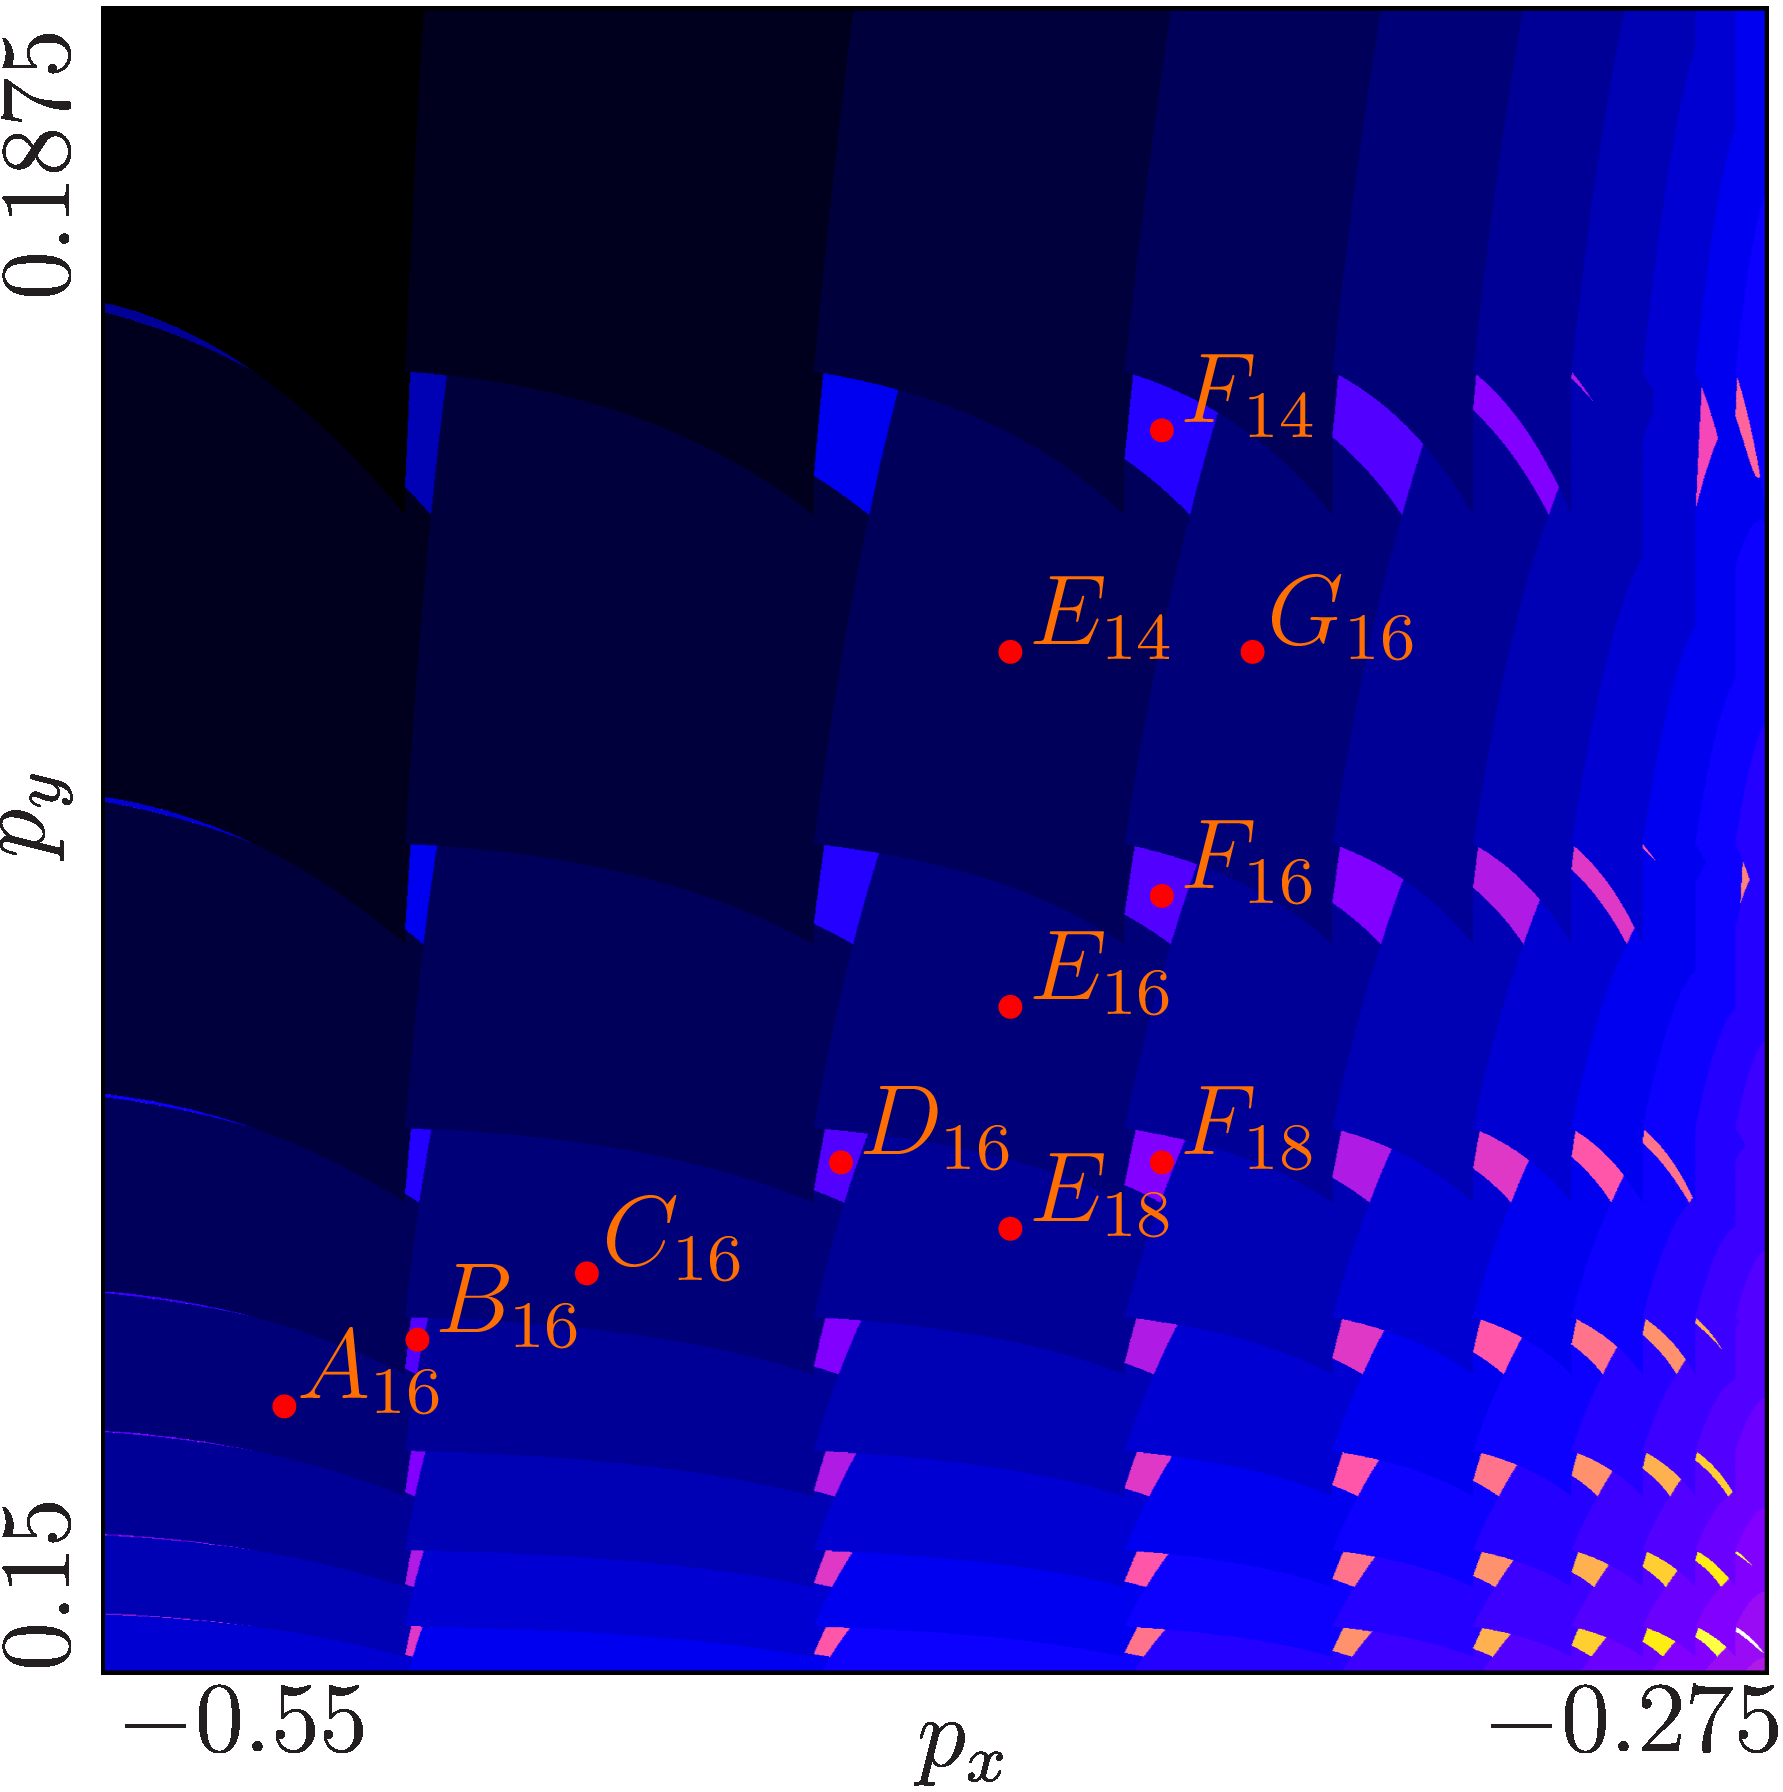
\includegraphics[height=0.6\textheight]{60_MinimalRepr/2D_Period_Whole_Lotta_Points/result-halved.png}}
        \caption{2D Scans of Periods of Minimal Reproducing Model}
    \end{figure}
\end{frame}

\begin{frame}{Minimal Reproducing Model Dynamics}
    \begin{figure}
        \centering
        \subfloat[At Point $C_{16}$]{\includegraphics[height=0.6\textheight]{60_MinimalRepr/Cobweb_C16/result.png}}
        \subfloat[At Point $D_{16}$]{\includegraphics[height=0.6\textheight]{60_MinimalRepr/Cobweb_D16/result.png}}
        \subfloat[At Point $E_{16}$]{\includegraphics[height=0.6\textheight]{60_MinimalRepr/Cobweb_E16/result.png}}
        \caption{Cobwebs}
    \end{figure}
\end{frame}

\begin{frame}{Parameter Regions in Original Model}
    \begin{itemize}
        \item ``Type A'': At points $C_{16}$ and $E_{16}$ in 2D scan
              \begin{itemize}
                  \item One cycle
                  \item Symmetrical
                  \item Example at point $C_{16}$: $\Cycle{\A^6\B^2\C^6\D^2}$
                  \item Example at point $E_{16}$: $\Cycle{\A^5\B^3\C^5\D^3}$ \vspace*{1em}
              \end{itemize}
        \item ``Type B'': At point $D_{16}$ in 2D scan
              \begin{itemize}
                  \item Two coexisting cycles
                  \item Asymmetrical
                  \item Example at point $D_{16}$: $\Cycle{\A^6\B^2\C^5\D^3}$ and $\Cycle{\A^5\B^3\C^6\D^2}$
              \end{itemize}
    \end{itemize}
\end{frame}

\begin{frame}{Definition of Minimal Reproducing Model (1/2)}
    \vspace{-3.0em}
    \begin{align}
        x \mapsto f(x) \mod 1
    \end{align}

    \begin{align}
        f(x) & = \begin{cases}
                     g(x)                                        & \text{ if } x < \frac{1}{2} \\
                     g\left(x - \frac{1}{2}\right) + \frac{1}{2} & \text{ else}
                 \end{cases}
    \end{align}

    \begin{align}
        g(x) & = \begin{cases}
                     l(x) & \text{ if } x < \frac{1}{4} \\
                     r(x) & \text{ else}
                 \end{cases}
    \end{align}
\end{frame}

\begin{frame}{Definition of Minimal Reproducing Model (2/2)}
    \vspace{-3.0em}
    \begin{align}
        l(x) & = a_L \cdot t_L(x)^2 + b_L \cdot t_L(x) + c_L
    \end{align}

    \begin{align}
        r(x) & = b_R \cdot t_R(x) + c_R
    \end{align}

    \begin{align}
        s(x)   & = x \mod 1            \\
        t_L(x) & = s(x) - \dfrac{1}{8} \\
        t_R(x) & = s(x) - \dfrac{3}{8}
    \end{align}
\end{frame}